\RequirePackage{graphicx}
\documentclass{beamer}

\usepackage{enumerate}
\usepackage{color}
\usepackage{beamerthemesplit}
\usepackage{graphicx}
\usepackage{epstopdf}
\DeclareGraphicsExtensions{.tiff, .jpg, .png}
\newcommand{\union}{\bigcup}
\newcommand{\intersect}{\bigcap}
\newcommand{\QED}{\blacksquare}
\newcommand{\homo}{\simeq}
\newcommand{\A}{\big(A_1,\ldots,A_m\big)}
\newcommand{\R}{\mathbb{R}}
\newcommand{\Z}{\mathbb{Z}}
\newcommand{\Q}{\mathbb{Q}}
\newcommand{\N}{\mathbb{N}}
\newcommand{\C}{\mathbb{C}}
\newcommand{\h}{\mathbb{H}}
\newcommand{\T}{\mathcal{T}}
\newcommand{\s}{\mathcal{S}}
\newcommand{\E}{\mathcal{E}}
\newcommand{\F}{\mathcal{F}}
\newcommand{\p}{\mathcal{P}}
\newcommand{\w}{\mathcal{W}}
\newcommand{\ov}{\overline}
\newcommand{\comp}{\overline}
\newcommand{\snd}{\Sigma_{n,d}}
\newcommand{\pnd}{\R[x_1,\ldots,x_n]_{2d}}
\newcommand{\pn}{\R[x_1,\ldots,x_n]}

\DeclareMathOperator{\trace}{trace}
\DeclareMathOperator{\kernel}{ker}
\DeclareMathOperator{\conv}{conv}
\DeclareMathOperator{\rank}{rank}
\DeclareMathOperator{\co}{co}

\newcounter{qcounter}

\title{Quadratic Convexity and Sums of Squares}
\author{Martin Ames Harrison}
\date{October 25, 2013}

\begin{document}

\frame{\titlepage}

\frame
{
\frametitle{Overview}
\begin{itemize}
\item<1->{\bf Introduction}
\begin{itemize}
\item Motivation
\item Terms and problem statement
\item Tools: matrices and convexity
\end{itemize}
\item<2->{\bf Main Results}
\begin{itemize}
\item Reformulation and related problems
\item Quadratic maps in general
\item	 Necessary condition
\end{itemize}

\item<3->{\bf Back to SOS}
\begin{itemize}
\item Application
\item Conjecture
\end{itemize}
\end{itemize}

}

\frame
 {
 \frametitle{Introduction - Why SOS?}
 
 Characterizations of positive polynomials allow polynomial optimization because
 \[\inf \{p(x) \mid x \in C\} = \sup \{y \mid (p-y)|_C > 0\}.\]
 \pause Positive polynomials can be described in terms of sums of squares.\\
 \vspace{.5cm}
 \pause SOS approximations are easy to find.\\
 }



%%%Introductory Frame%%%
\frame
{
  \frametitle{Introduction - Notation}
  \begin{itemize}[<+->]
   
   \item $\pn_d$ is the space of real homogeneous polynomials in the variables $x_1,\ldots,x_n,$ of degree $d$ (plus $0$).
   \item For a multi-index $\alpha = (\alpha_1,\ldots,\alpha_n) \in (\N \cup \{0\})^n$, $x^\alpha=x_1^{\alpha_1}\cdots x_n^{\alpha_n}$.
   \item $\snd$ denotes the SOS \emph{cone}, sums of squares in $\pnd$, i.e.
   \[g_1^2+\ldots+g_k^2\]
   for some $g_1,\ldots,g_k \in \pn_{d}$ (necessarily).
   \item Degree of $x^\alpha$ is $|\alpha| \equiv \sum_j \alpha_j$.
   \item For $k\in \N$, $\snd(k)$ is the set of sums of $k$ (or fewer) squares. 
    
 \end{itemize}
 }
 
  
 
 %%%Basic Example Frame%%%
 \frame
 {
 \frametitle{Introduction - Example }
The polynomial $p(x,y) = x^4+x^2y^2+y^4$ is a sum of $3$ squares:
\[p(x,y) = (x^2)^2 + (xy)^2 + (y^2)^2\]
\pause
Will fewer squares suffice? \pause Yes!
\[p(x,y) = (x^2-y^2)^2+(\sqrt{3}xy)^2\]
Will \emph{even fewer} suffice? \pause No! The length of $p(x,y)$ is $2$.
 
 }
 %%%Basic Question%%%
 \frame
 {
 \frametitle{Introduction - Problem}
 \begin{itemize}[<+->]
 \item The {\color{cyan}length} of $\sigma \in \snd$ is the smallest natural number $k$ for which $\sigma \in \snd(k)$. We write $\ell(\sigma)$ for the length of $\sigma$.
 \item The {\color{cyan}pythagoras number} $\p(S)$ of a set $S \subseteq \pnd$ is the maximum of the set $\{ \ell(\sigma) \mid \sigma \in S\}$. Equivalently, the smallest $k$ for which $\snd(k) = \snd$.
 \item Known: $\p(\Sigma_{2,d})=2$, $\p(\Sigma_{n,1})=n$  and $\p(\Sigma_{3,2})=3$.
 \end{itemize}
 
 \onslide<+->
 {
 {\color{magenta}\emph{ How does one compute $\p(\snd)$?}}
 }
 }
 
 
 
 \frame
{
\frametitle{Introduction - Convexity} 
\begin{itemize}[<+->]
\item A subset $S$ of a real vector space is called {\color{cyan}convex} if for all $t \in [0,1]$ and all $x,y \in S$, $tx+(1-t)y$ belongs to $S$.
\item A {\color{cyan}convex combination} takes the form $t_1x_1+\ldots+t_kx_k$, where $x_i$ are vectors and $t_i\geq0$ sum to $1$.
\item The {\color{cyan}convex hull} $\conv(S)$ of a set $S$ is the smallest convex set containing $S$; all convex combinations of elements of $S$.
\item The {\color{cyan}conic hull} $\co(S)$ is the set of all {\color{cyan}conic combinations} of elements of $S$: \[\co(S) = \{ t_1x_1+\ldots+t_kx_k \mid x_i \in S, t_i \geq 0\}.\]
\end{itemize}
} 

\frame
{
\frametitle{Carath\'{e}odory Convex Hull Theorem}
If $S \subset \R^{\color{red}d}$, then every element of $conv(S)$ may be expressed as a convex combination of ${\color{red}d}+1$ or fewer elements of $S$. \pause
\begin{figure}[H]
  
  \begin{center}
    
\includegraphics[width=0.5\textwidth]{Caratheodory}
    
    \label{Caratheodory}
  \end{center}
\end{figure}

}


\frame
{
\frametitle{Separating Hyperplane}
If $C\subset \R^m$ is a closed convex set and $x \notin C$, then there is an affine hyperplane strictly separating $x$ and $C$.\\ \pause 

That is, there exists a linear functional $\Lambda$ on $\R^m$ and a real number $r$ such that $\Lambda(y) < r$ for all $y\in C$ and $\Lambda(x) > r$.\\ \pause
\begin{columns}
    \begin{column}{0.5\textwidth}
      \centering
      \includegraphics[width = 5 cm]{SeparatingLine}
    \end{column}\pause
    \begin{column}{0.5\textwidth}
      \centering
      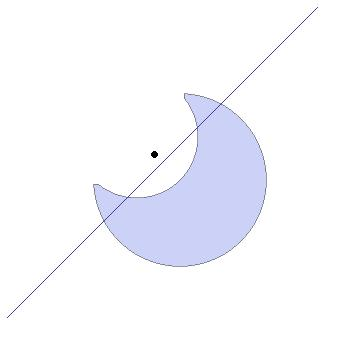
\includegraphics[width = 5 cm]{SeparationFailed}
    \end{column}
  \end{columns}
 }

\frame
{
\frametitle{A special property}
Let $S\subset \R^m$ be a convex set. If $\mathring{S} = \emptyset$, then $S$ is contained in a proper affine subspace of $\R^m$.
}
  
 
 \frame
{
\frametitle{Introduction - PSD matrices}
The algebra of $N\times N$ matrices over $\R$ is denoted by $M_N(\R)$.\\
\pause
The set $\s_N\subseteq M_N(\R)$ consists of the symmetric matrices.\\
\pause
If $A\in\s_N$ has only nonnegative eigenvalues, then we write $A \in \s_N^+$ and $A \succeq 0$, and we call $A$ {\color{cyan}positive semidefinite}.\\
\pause
For $A \in \s_N$, the following are equivalent:
\begin{list}{\roman{qcounter})}{\usecounter{qcounter}}
\item $A$ is positive semidefinite.
\item $A = B^2$ for some $B \in \s_N$.
\item $x^TAx \geq 0$ for all $x \in \R^N$.
\item The principal minors of $A$ are nonnegative.
\item $A=LL^T$ for some $L \in M_N(\R)$.
\end{list}
\pause 
Finally, $K_N^+\equiv \s_N^+ \cap \{x \in M_N(R) \mid \trace (x)=1\}$ (example of a {\color{cyan}spectrahedron}).

} 

\frame
 {
 \frametitle{PSD matrices and SOS}
 %Mention something about SDP and spectrahedra
 \begin{itemize}[<+->]
 \item Fix $p = \sum_\alpha p_\alpha x^\alpha = g_1^2+\ldots+g_k^2$.
 \item $g_i=\sum_\alpha g_{i,\alpha}x^\alpha$
 \item ${\bf g_i} \equiv (g_{i,\alpha})_{|\alpha|=d}^T \in \R^N$ and ${\bf m} = (x^\alpha)_{|\alpha|=d}^T \in \pn_d^N$
 \item $g_i^2 = {\bf g_i}^T {\bf m} {\bf m}^T {\bf g_i}=\trace( {\bf g_i}{\bf g_i}^T{\bf m}{\bf m}^T)$, and
 \item $p = \trace({\bf m}{\bf m}^T(\sum_i{\bf g_i}{\bf g_i}^T))$.
 \item System of $\binom{n+2d-1}{2d}$ equations $p_\alpha = \trace(A_\alpha \sum_i{\bf g_i}{\bf g_i})$, where

\[(A_\alpha)_{\beta,\gamma} = 
\begin{cases}
1, & \text{if }\beta+\gamma=\alpha \\
0, & \text{otherwise }
\end{cases}
\]
 \end{itemize}
 }
 
 \frame
 {
 \frametitle{PSD matrices and SOS}
 \begin{itemize}[<+->]
 \item $\sum_i{\bf g_i}{\bf g_i}^T$ is positive semidefinite
 \item Conversely, $X \in \s_N^+$ satisfying $p_\alpha = \trace(A_\alpha X)$ yields a sum of squares. Write $U^TDU=X$.
 
\[p =\trace({\bf m}{\bf m}^TX)= \trace({\bf m}^TU^TDU{\bf m})=\sum_i \lambda_i (U_i{\bf m})^2\]
 
 \item $\ell(p) = \min \{\rank(X)\mid X \in S(p)\}$, where $S(p)$ is the set of all Gram matrices for $p$.
 \item $\p(\snd) \leq \binom{n+d-1}{d}$
 \end{itemize}
 
 }
 
 \frame
 {
 \frametitle{Quadratic Maps}
 $A=(A_1,\ldots,A_M)$,  $M-$tuple of elements of $\s_N$\\
 \vspace{.5cm}
 $A(x)\equiv(x^TA_1x,\ldots,x^TA_Mx)^T\in \R^M$, $A$ is a quadratic map.
 
 \begin{itemize}[<+->]
 \item When is $A(\R^N) \equiv \{(x^TA_1x,\ldots,x^TA_Mx) \mid x\in \R^N\}$ convex?
 \item When is $A(S^{N-1}) \equiv \{(x^TA_1x,\ldots,x^TA_Mx) \mid x\in S^{N-1}\}$ convex?
 \item Who cares, and what does this have to do with pythagoras numbers?
 \end{itemize}
 }
 
\frame
{
\frametitle{Quadratic Convexity - motivation}
\begin{itemize}[<+->]
\item Relaxation of systems of quadratic equations
\[x^TA_ix = a_i\]
$a=(a_1,\ldots,a_M)$ outside the convex hull of $A(\R^N)$ can be separated by a hyperplane...
\item SDP - find $y$ such that 
\[y_1(A_1-a_1I)+\ldots+y_M(A_M-a_MI)\succ0\]
\item Joint numerical range of a tuple of hermitian operators - applications in \emph{quantum} physics
\[w(A) = \{(z^*A_1z,\ldots,z^*A_Mz)\mid z\in \C^N \text{ and } \|z\|=1\}\]
\end{itemize}
}

\frame
{
\frametitle{Quadratic Convexity - pythagoras numbers}
\begin{itemize}[<+->]
\item $\snd(k)$ is the image of a quadratic map
\item $I_k\otimes A \equiv (I_k \otimes A_\alpha )_{|\alpha|=2d}$, where $I_k$ is the $k\times k$ identity matrix and $\otimes$ is the Kronecker product.
\item The set $\snd(k)$ is convex exactly when 
\[\snd = \snd(k),\]
i.e., exactly when $\p(\snd)\leq k$.
\end{itemize}
}



\frame
 {
 \frametitle{Quadratic Convexity - first observations}
 \emph
 {
 Suppose that $A : \R^N \to \R^M$ is a quadratic map. Let $\mathbb{B}$ denote the unit ball $\{x \in \R^N \mid \|x\| \leq1\}$ in $\R^N$. \\
 \vspace{.5cm}
 Then $A(\R^N)$ is convex whenever $A(\mathbb{B})$ is convex, and $A(\mathbb{B})$ is convex whenever $A(S^{N-1})$ is convex.\\
 \vspace{.5cm}
 \pause
 }
 The converses are false, but we can reduce the question to one about a \emph{compact} set.
 
 }



 \frame
 {
 \frametitle{Quadratic Convexity - Positive maps}
Suppose $A : \R^N \to \R^M$ is a quadratic map and $A(\R^N)$ spans $\R^M$. TFAE
\begin{list}{\roman{qcounter})}{\usecounter{qcounter}}
\item $0 \notin A(K_N^+) \equiv \conv A(S^{N-1})$
\item There is a linear functional $\ell$ on $\R^M$ such that $\ell \cdot A \equiv \sum_j \ell_j A_j$ is positive definite.
\item There is an invertible linear operator $T$ on $\R^M$ such that $T\circ A$ is positive definite in each coordinate.
\end{list}
 }
 
 \frame
 {
 \frametitle{Positive maps - Corollary}
 \begin{itemize}[<+->]
 \item 
 \emph
 {
 Suppose that $A : \R^N \to \R^M$ is a quadratic map and $\conv A(S^{N-1})$ does not contain $0$.\\
 \vspace{.5cm}
  Then there is an invertible linear operator $L$ on $\R^N$ such that $A(\R^N)$ is convex exactly when $A \circ L(S^{N-1})$ is convex.
  \vspace{.5cm}
 }
 \item
 \emph
 {
 If $A(\R^N)$ is closed and contains no lines, then there is a linear transformation $T$ from $\R^k$ to $\R^N$, for some $k \leq N$, such that $A(\R^N)$ is convex exactly when $A\circ T(S^{k-1})$ is convex.
  }
 \end{itemize}
 }
 
 \frame
 {
 \frametitle{Quadratic Convexity - A rank condition}
 %Explain here the rank condition and how it can be distilled to the nonzeroness of that retarded polynomial.
 \begin{itemize}[<+->]
 \item Recall a property of convex sets: nonempty interior \emph{or} lower dimension
 \item Sard's Theorem: Critical values have measure zero. 
 \item A quadratic map is polynomial, and so is the derivative.
 \end{itemize}
 
 }





\frame
{
\frametitle{Quadratic Convexity - Squashing images}
\emph
{
If $A : \R^N \to \R^M$ is a quadratic map, then...\\
\vspace{.5cm}
there is a linear operator $T:\R^M\to \R^k$ satisfying
\begin{list}{\roman{qcounter})}{\usecounter{qcounter}}
\item $(T \circ A)(\R^N)$ is contained in no proper subspace of $\mathbb{R}^k$, and
\item $(T \circ A)(\R^N)$ is convex if and only if $A(\R^N)$ is convex.
\end{list} 
\vspace{.5cm}
\pause
there is a linear operator $T:\R^M\to \R^k$ satisfying
\begin{list}{\roman{qcounter})}{\usecounter{qcounter}}
\item $(T \circ A)(S^{N-1})$ is contained in no proper affine subspace of $\mathbb{R}^k$, and
\item $(T \circ A)(S^{N-1})$ is convex if and only if $A(S^{N-1})$ is convex.
\end{list}
}
}
\frame
{
\frametitle{SOS revisited}
% Explain here how the nonzeroness of the polynomial lets us determine a lower bound on the pythagoras number AND how it lets us determine the smallest number occurring as the pythagoras number of an open set.
% 
% Also conjecture that this in fact gives the pythagoras number.
% Also note that SOS is closed and contains no lines.
%Note that the set of single squares spans the entire space.
}
  
 
 
 
 
 
 
 \frame
 {
 \frametitle{Summary}
 \begin{itemize}[<+->]
 \item Convexity of a quadratic image equivalent to that of a \emph{compact} set
 \item Necessary condition on rank of derivative, applicable to all quadratic maps after modification
 \item Lower bounds on pythagoras numbers, smallest pythagoras number of a nonempty open subset
 \end{itemize}
 }
 
 
 
 
 
%\begin{thebibliography}{9}
% 
%\bibitem{BochAlg}
%  J. Bochnak, M. Coste, M-F. Roy,
%  \emph{G\'{e}om\'{e}trie alg\'{e}brique r\'{e}elle}.
%  Springer-Verlag, Berlin and Heidelberg,1987.
%  
% \bibitem{Helt} 
% J. W. Helton,
%\emph{``Positive" noncommutative polynomials are sums of squares.}  Ann. of Math. (2) 156 (2002), no.2, 675-694.
%
%\bibitem{Prestel}
%A. Prestel,
%\emph{Positive polynomials: from Hilbert's $17^{th}$ problem to real algebra.} Springer, Berlin and New York, 2001.
%
%\bibitem{HeltPut}
%J.W. Helton, S. McCullough, M. Putinar,
%\emph{Matrix representation for positive non-commutative polynomials}, Positivity 10(2006), 145-163.
%
%\bibitem{Faz}
%M. Fazel, B. Recht, P. Parrilo,
%\emph{Guaranteed Minimum-Rank Solutions of Linear Matrix Equations 
%via Nuclear Norm Minimization}, preprint (2008).
%
%\bibitem{Tao}
%E. J. Cand\'{e}s. 
%\emph{Compressive sampling}. In International Congress of Mathematicians. Vol. III, pages 
%1433�1452. Eur. Math. Soc., Zurich, 2006. 
%
%
%
%
%
%\end{thebibliography}




















 \end{document} 